\documentclass[a4paper,10pt]{article}
\usepackage[top=3.5cm,bottom=2cm,left=2cm,right=2cm,headsep=1cm,footskip=1.2cm]{geometry}
\usepackage{fontspec,xeCJK}
\IfFontExistsTF{Times New Roman}{\setmainfont{Times New Roman}}{\setmainfont{texgyretermes}[Extension=.otf,UprightFont=*-regular,ItalicFont=*-italic,BoldFont=*-bold,BoldItalicFont=*-bolditalic]}
\IfFontExistsTF{Songti TC}{\setCJKmainfont{Songti TC}}{\setCJKmainfont{FandolSong-Regular.otf}[BoldFont=FandolSong-Bold.otf]}
\usepackage{amsmath,amssymb,booktabs,array,multicol,tikz,caption,titlesec,fancyhdr,enumitem}
\usepackage[hidelinks]{hyperref}
\usetikzlibrary{arrows.meta,positioning}
\setlength{\columnsep}{0.748cm}
\setlength{\parindent}{1.5em}
\setlength{\parskip}{0pt}
\renewcommand{\normalsize}{\fontsize{9}{13.5}\selectfont}
\renewcommand{\small}{\fontsize{8}{12}\selectfont}
\renewcommand{\footnotesize}{\fontsize{8}{11}\selectfont}
\renewcommand{\thesection}{\Roman{section}}
\renewcommand{\thesubsection}{\arabic{subsection}}
\titleformat{\section}{\centering\fontsize{11}{16.5}\bfseries}{\thesection.}{0.5em}{}
\titleformat{\subsection}{\normalsize\bfseries}{\thesubsection.}{0.5em}{}
\titlespacing*{\section}{0pt}{12pt}{6pt}
\titlespacing*{\subsection}{0pt}{8pt}{3pt}
\captionsetup{font=small,labelfont=bf,labelsep=period}
\setlist{nosep,leftmargin=*}
\pagestyle{fancy}\fancyhf{}\fancyfoot[C]{\small\thepage}
\renewcommand{\headrulewidth}{0pt}
\setlength{\emergencystretch}{1.5em}
\newcommand{\sg}{\operatorname{sg}}
\newcommand{\AP}{\operatorname{AP}}
\begin{document}\normalsize
\begin{center}
{\fontsize{18}{23}\selectfont\bfseries Gradient Routing and Temporal State in Inductive Link Prediction:\\ A Controlled Study of Decoupled SR-GNN\par}
\vspace{12pt}
{\fontsize{10}{15}\selectfont Duong Viet Hoang\textsuperscript{a,*}, Duong Viet Huy\textsuperscript{b}, Lun-Min Shih\textsuperscript{a}\par}
\vspace{6pt}
{\itshape\textsuperscript{a}Department of Computer Science, Da-Yeh University, Changhua, Taiwan\\
\textsuperscript{b}Department of Computer Science, Kent State University, Ohio, United States\par}
\vspace{6pt}
*Corresponding author: \href{mailto:Hoangduong4316@icloud.com}{Hoangduong4316@icloud.com}
\end{center}
\vspace{18pt}
\begin{center}\fontsize{11}{16.5}\selectfont\bfseries ABSTRACT\end{center}
\begin{list}{}{\setlength{\leftmargin}{2cm}\setlength{\rightmargin}{2cm}}\item[]
Inductive temporal link prediction requires a model to score interactions involving entities absent from earlier observations. Jointly optimizing a temporal representation and its link readout is a natural design choice, but it need not be the most effective choice for a particular inductive protocol. This study investigates gradient routing in SR-GNN, a temporal model combining event encoding, recurrent node memory, deterministic pair-history signals and a hierarchical readout. We specify the scored gradient boundary, distinguish parameter learning from event-state evolution, and compare coupled and decoupled versions of the same registered readout. A separate freeze-then-probe procedure examines a different training trajectory. Experiments use chronological partitions of CoEdit, Wikipedia and MOOC and a fixed random-destination evaluation procedure. Checksum-bound results are reported as mean inductive average precision and sample standard deviation across the registered seeds. The observed decoupled arm has higher mean inductive average precision than the coupled arm on each corpus. This supports a bounded within-protocol comparison rather than a general claim that end-to-end learning is harmful. The analysis identifies important interpretation limits: CoEdit shares its source with Wikipedia, its event construction includes retrospective information, the candidate sampler is not destination-type constrained, and temporal memory follows mixed batch and sequential semantics. Historical experiments are reconciled at the level of configuration identity but are not pooled with the current results. The study contributes an explicit account of gradient routing and temporal evaluation that makes the observed comparison reproducible and its scope assessable.

\vspace{10pt}\noindent\textbf{Key words:} temporal graphs, inductive link prediction, gradient decoupling, recurrent memory, reproducible evaluation
\end{list}
\clearpage
\begin{multicols}{2}
\section{Introduction}
Temporal graphs describe relationships through ordered interactions rather than a single static adjacency matrix. An edit on a collaborative platform or an action in an online course supplies information about both the participating entities and their recent activity. Predicting an interaction therefore involves a representation of evolving history, a candidate-scoring rule, and a decision about which historical information is available at the prediction time. These components jointly define the learning problem. A change to event ordering or candidate construction can alter the meaning of a reported score even when the neural architecture is unchanged.

Inductive prediction adds another constraint: some evaluated interactions involve entities absent from the training population. A model cannot rely solely on well-trained representations of those entities. Shared encoders, temporal neighborhoods, pair statistics and initialization rules become relevant to transfer. Nevertheless, inductive evaluation is not a unique protocol. The treatment of validation entities, the handling of preceding test events and the membership of negative-candidate pools all determine what a new entity means operationally. We state these choices explicitly instead of using the word inductive as a sufficient description of the experiment.

Most task-trained representations allow prediction gradients to update the encoder that produces their features. This gives the encoder a direct way to preserve information useful for the training objective. It can also create a dependence on the training population and on the particular candidate-sampling distribution. Stopping a scored gradient changes this optimization pressure while retaining the representation's forward value. The resulting tradeoff is empirical: reducing task adaptation can either preserve transferable information or remove a useful learning signal. Neither outcome follows from the stop-gradient operation alone.

Temporal methods make this question especially interesting because they combine learned weights and evolving state. A detached representation is not necessarily static. Node memories can change during forward execution, pair statistics can accumulate observations, and auxiliary objectives can update parameters outside the detached scoring path. Calling the entire model frozen would conflate these mechanisms. Conversely, freezing an encoder after pretraining does not recreate the trajectory obtained by preventing a scored gradient from reaching it throughout initial training.

We study this distinction in SR-GNN, the implementation provided by the accompanying research repository \cite{repo}. Its temporal representation combines an event encoder, recurrent node memory and a bank of pair-history signals. A hierarchical readout produces the scored link output. The primary experiment changes whether that readout receives detached features while preserving the registered readout configuration. A separate freeze-then-probe arm uses pretraining followed by a newly initialized prediction head. These are deliberately interpreted as different experimental procedures.

The paper develops three connected contributions. First, it specifies the gradient boundary mathematically and separates the derivative of the scored output from other gradient paths. Second, it documents the temporal state and evaluation semantics required to interpret that boundary in a stateful model. Third, it reports a checksum-bound within-protocol comparison in which the decoupled arm has higher mean inductive average precision on each registered corpus. The contribution is this controlled observation and its operational specification. It is not a new stop-gradient primitive, a faithful external-model ranking, or proof of a universal mechanism.

The remainder of the paper places the study in the temporal-learning and representation-learning literature, defines the model and optimization contrast, specifies the data and evaluator, and presents the current results. The discussion then examines competing explanations and the relationship between the current experiment and earlier configurations. This organization separates what the computation guarantees from what the experiment measures and from what remains a hypothesis.

\section{Related Work}
\subsection{Memory and temporal-neighborhood models}
JODIE models the co-evolution of interacting entities through dynamic embedding trajectories and provides the public interaction sources used in this study \cite{jodie}. DyRep studies representation learning over dynamic graphs with a temporal point-process formulation \cite{dyrep}. Temporal Graph Networks provide a framework combining memory, message functions and temporal graph computation \cite{tgn}. Their differing state-update mechanisms illustrate that temporal history can enter a prediction through several computational routes. They motivate the need to specify both the learned representation and its update schedule.

These models should not be treated as interchangeable implementations of a generic memory baseline. The definition of a message, the timing of memory updates, the sampling of neighbors and the construction of the predictor are part of the model. A local approximation can be useful for debugging or controlled exploration, but its result cannot inherit the identity or performance interpretation of the published architecture. The current empirical comparison consequently concerns registered SR-GNN arms rather than a ranking of simplified implementations carrying familiar model names.

TGAT constructs temporal representations through attention over time-dependent neighborhoods \cite{tgat}. Causal anonymous walks provide an alternative route to inductive representation learning that emphasizes temporally ordered structural patterns \cite{cawn}. GraphMixer investigates a simpler architecture built from multilayer perceptrons and neighborhood aggregation \cite{graphmixer}. These approaches show that persistent recurrent memory is not the only way to represent temporal structure. They also suggest possible future tests of gradient routing, provided a corresponding intervention is defined within each architecture.

More recent approaches examine richer representations of neighborhood relations and interaction histories. NAT uses dictionary-based neighborhood representations to construct structural features efficiently \cite{nat}. TCL studies transformer-based dynamic graph modeling through contrastive learning \cite{tcl}. DyGFormer uses a transformer architecture and is presented with DyGLib, a unified library for dynamic graph learning \cite{dygformer}. These works broaden the available design space. They do not establish that the particular routing result observed here transfers to their encoders or training objectives.

\subsection{Evaluation and candidate distributions}
Evaluation methodology is central to temporal link prediction. Poursafaei et al. examine dynamic link prediction under different negative-sampling strategies and introduce EdgeBank as a memorization-based comparator \cite{poursafaei}. The Temporal Graph Benchmark develops a standardized setting for evaluating learning on temporal graphs \cite{tgb}. Together these contributions motivate reporting the candidate population and historical information available to a model, rather than treating a high aggregate score as sufficient evidence of a generally useful predictor.

A negative candidate is normally an unobserved or sampled alternative, not a verified impossible interaction. Its difficulty depends on whether the pair has interacted before, whether its endpoints are valid for the domain, and whether the model has already seen those endpoints. A random node from the wrong endpoint type can be much easier to distinguish than a plausible alternative item. Likewise, historical and test-only pair pools probe different behavior from uniform random destinations. A shared sampler improves internal comparability, but does not make these distinct populations equivalent.

Our main result is restricted to the registered random-destination evaluator. The accompanying historical archive contains harder-negative experiments, but their configuration and execution identities differ from those of the current matrix. They are useful for reconstructing the development of the study. They are not combined with the present table to imply robustness across candidate regimes. A future evaluation should align the source, data and model identities before making that extension.

\subsection{Gradient separation and representation transfer}
The use of an independently trained probe to examine a representation predates this study. Alain and Bengio investigate intermediate neural representations through linear classifier probes \cite{alain}. Kumar et al. analyze circumstances in which fine-tuning can distort pretrained features and underperform linear probing out of distribution \cite{kumar}. These results make representation adaptation a legitimate object of study, but they do not imply that a temporal representation exposed to a link objective is irreparably damaged. That stronger conclusion would require a specified recovery criterion and substantially broader interventions.

Stop-gradient also appears in self-supervised representation learning. Chen and He study its role in a simple Siamese learning method \cite{simsiam}, while Caron et al. investigate self-distillation for vision transformers \cite{dino}. Their objectives and training systems differ from the temporal supervised setting considered here. The relevant connection is a computational one: controlling which objective updates which component can change representation learning. We do not transfer their guarantees or empirical outcomes to temporal link prediction.

The information bottleneck offers a framework for discussing information retained in a representation \cite{tishby}. Variational formulations connect such ideas to tractable neural objectives \cite{alemi}; variational auto-encoding provides another important foundation for latent-variable regularization \cite{vae}. These works motivate the use of a variational penalty, but a penalty's presence is not a measurement of identity information or proof that nuisance information has been removed. We therefore distinguish a regularization objective from an empirical mechanism claim.

\subsection{Online pair-history features}
Pair recurrence and elapsed-time statistics provide information that is complementary to a learned node memory. Hawkes processes give a classical model of self-exciting event behavior \cite{hawkes}. Welford's recurrence provides a numerically stable way to update running moments \cite{welford}. SR-GNN uses intensity-like and online-moment channels inspired by these ideas, together with rate and recurrence summaries. The channels are features of the implemented scoring system; the present study does not fit or validate a standalone generative Hawkes process.

The distinction between a statistical feature and a generative model is consequential. A feature can improve discrimination without being a calibrated conditional intensity. Its usefulness also depends on how timestamps and gaps are constructed. We specify the actual updates and their temporal availability below. This prevents the interpretation of an intensity-like channel from carrying assumptions that the evaluation has not tested.

\section{Problem and Model Specification}
\subsection{Events, candidates and information}
Let an event stream contain tuples $e_i=(u_i,v_i,t_i,x_i)$ in nondecreasing timestamp order. The vector $x_i$ contains attributes supplied by the data pipeline. Let $\mathcal H_i$ denote the history retained by the particular training or evaluation pass immediately before scoring event $i$. It need not equal the full raw stream prefix: filtering an evaluation stream before execution changes the observations that enter its state. The model assigns a score to a candidate pair conditioned on this retained history and on the supplied attributes.

We write the temporal representation and output as
\begin{align}
h_i&=F_\theta(u_i,v_i,t_i,x_i;\mathcal H_i),\nonumber\\
p_i&=\sigma(G_\psi(h_i,\phi_i)),
\label{eq:model}
\end{align}
where $\theta$ and $\psi$ denote backbone and readout parameters, respectively, and $\phi_i$ denotes the available pair-history context. This decomposition names the scored boundary; it is not an assertion that every auxiliary quantity is independent of every parameter in $F_\theta$. In the implementation, candidate-specific positive and negative branches have corresponding representations and histories.

The distinction between weights and state is essential. Parameters are updated by the optimizer. Node memory, pair counters and other stores are updated by event execution. A parameter can remain fixed while the state used by its forward computation changes. Similarly, a stop-gradient can prevent a backward update without removing information that entered the forward state through earlier observations. Inductive behavior depends on both mechanisms.

\subsection{Deterministic pair-history updates}
For an ordered pair, let $g_k$ be the gap supplied to its deterministic update at its $k$th retained observation. Denote the running mean by $\mu_k$ and the sum of squared deviations by $M_k$. The online moment recurrence is
\begin{align}
\delta_k&=g_k-\mu_{k-1},\nonumber\\
\mu_k&=\mu_{k-1}+\delta_k/k,\nonumber\\
M_k&=M_{k-1}+\delta_k(g_k-\mu_k).
\label{eq:welford}
\end{align}
The feature variance is formed from the accumulated moments using the implementation's population-moment convention. This within-pair feature variance must not be confused with the sample standard deviation across independent training seeds used in the result table. The two quantities answer different questions and have different denominators.

In the current forward implementation, the supplied gap is source-node staleness from the node-memory store. It is not necessarily the elapsed time since the same pair last interacted. The statistics are indexed by pair but accumulate this supplied gap. This distinction limits a literal interpretation as inter-arrival moments of a pair-specific point process.

The recurrence and intensity-like updates can be expressed as
\begin{align}
r_k&=a+(1-a)r_{k-1}\exp(-\eta g_k),\label{eq:recurrence}\\
\ell_k&=\mu_0+(\ell_{k-1}-\mu_0)\exp(-\beta g_k)+\alpha.
\label{eq:hawkes}
\end{align}
Here $r_k$ summarizes recent recurrence, $\ell_k$ is the intensity-like channel, and the constants govern decay and event increments. Equation~\eqref{eq:hawkes} includes the baseline and event increment. Omitting either would describe a different update law. The resulting quantity is used as model context rather than reported as a calibrated event probability.

Fast and slow exponentially weighted rate estimates summarize changes in cadence. With $q_k=1/\max(g_k,\epsilon)$, their generic form is
\begin{align}
f_k&=a_fq_k+(1-a_f)f_{k-1},\nonumber\\
s_k&=a_sq_k+(1-a_s)s_{k-1}.
\label{eq:rates}
\end{align}
The gap floor keeps coincident observations finite. Relative fast and slow rates and a decaying rate peak provide additional context for the readout. Their values depend on time units and update ordering. These conventions must therefore travel with a result rather than being inferred from a feature name.

The model also maintains learned node-memory and pair-representation components. Deterministic statistics offer a direct summary of observations, whereas learned transformations can adapt how the summaries and event attributes are combined. Decoupling the scored path changes the latter adaptation without deleting the former information. This is why an effective detached arm does not imply that a random or history-free encoder would be equally effective.

\subsection{Readout and gradient boundary}
Let $D_0(h)=h$ and $D_1(h)=\sg(h)$, where stop-gradient is defined by its forward value and backward derivative:
\begin{equation}
\sg(h)=h,\qquad \frac{\partial\sg(h)}{\partial h}=0.
\label{eq:sg}
\end{equation}
The primary arms use the same registered readout family and differ in whether its scored feature input passes through $D_0$ or $D_1$:
\begin{equation}
p_i^{(d)}=\sigma\!\left(G_\psi(D_d(h_i),\phi_i)\right),
\quad d\in\{0,1\}.
\label{eq:arms}
\end{equation}
This boundary is applied to both positive and negative scoring branches. Detaching only observed interactions would leave a task-gradient route through the sampled negatives and would implement a different intervention.

For the path through $h_i$, the chain rule gives
\begin{equation}
\left.\nabla_\theta L_{\rm score}\right|_{h_i}
=\frac{\partial L_{\rm score}}{\partial G}
\frac{\partial G}{\partial D_d}
\frac{\partial D_d}{\partial h_i}
\frac{\partial h_i}{\partial\theta}.
\label{eq:chain}
\end{equation}
That contribution vanishes for the detached branch. This is a path-specific computational statement. It does not establish that every route from the complete weighted training objective to every backbone parameter vanishes. Additional dependencies through weights, shared modules or auxiliary losses must be inspected separately. In particular, the current soft-compliance weighting should not be silently treated as a detached constant when analyzing the entire objective.

\begin{center}
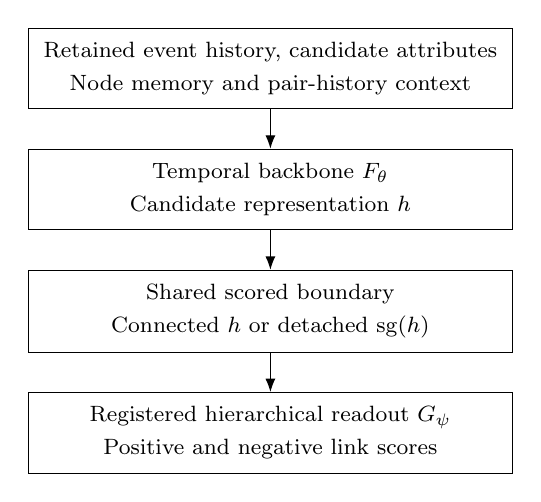
\begin{tikzpicture}[node distance=5mm,box/.style={draw,align=center,font=\small,text width=5.8cm,inner sep=5pt},>=Latex]
\node[box](hist){Retained event history, candidate attributes\\Node memory and pair-history context};
\node[box,below=of hist](enc){Temporal backbone $F_\theta$\\Candidate representation $h$};
\node[box,below=of enc](gate){Shared scored boundary\\Connected $h$ or detached $\sg(h)$};
\node[box,below=of gate](head){Registered hierarchical readout $G_\psi$\\Positive and negative link scores};
\draw[->](hist)--(enc);\draw[->](enc)--(gate);\draw[->](gate)--(head);
\end{tikzpicture}
\captionof{figure}{Scored feature path in the primary comparison.}
\end{center}
Figure~1 identifies the boundary changed by the experiment. Auxiliary objectives and deterministic store writes are not drawn as scoring edges. Their omission from this diagram is a visual simplification, not a claim that they are absent from training. The forward representations of arms with identical parameters would agree at the boundary, but their learned trajectories need not agree after optimization.

\subsection{Training objective and auxiliary routes}
For a scored logit $z$ and label $y$, the binary logistic loss is
\begin{equation}
\ell(z,y)=-y\log\sigma(z)-(1-y)\log(1-\sigma(z)).
\label{eq:bce}
\end{equation}
The implementation combines weighted per-example prediction losses with enabled auxiliary terms. A compact description is
\begin{equation}
L=\frac{1}{|\mathcal B|}\sum_{j\in\mathcal B}w_j\ell(z_j,y_j)
+\lambda_{\rm KL}L_{\rm KL}+\sum_{a\in\mathcal A}\lambda_aL_a.
\label{eq:loss}
\end{equation}
The auxiliary collection includes the active violation, transition, edge-state and entropy-related terms selected by the resolved profile. Disabled terms contribute nothing. The code, protocol and resolved configuration specify their actual inclusion and weights. Equation~\eqref{eq:loss} is a dependency summary rather than a substitute for that operational specification.

A useful distinction is between an unweighted scored-output gradient test and a test of the full training loss. The former can confirm a boundary property while the latter still has other routes into shared parameters. Reporting a successful test of the former as a guarantee about the latter would overstate its scope. Likewise, a variational penalty does not by itself prove that the representation retains only population-independent temporal information. The current experiment measures the outcome of a specified routing choice, not the information content of all learned features.

\subsection{State updates and batching}
Scoring and store mutation must be ordered consistently for positive and negative candidates. A positive candidate reads pre-update pair history; a negative candidate reads its own available pair history without inserting a fictional observation. Actual observations subsequently update the stores. If positives instead received their post-event counts while negatives saw only pre-event counts, the model could exploit an evaluation artifact rather than historical predictive information.

Repeated pairs within a batch require additional care. A single batch snapshot would expose the same old pair statistics to all repeated occurrences. The causal-batch option folds deterministic pair accumulators in stable event order so a later occurrence can read the state following an earlier occurrence in that batch. This addresses a store-level timing issue. It should not be interpreted as sequential execution of the entire neural model.

Recurrent node memory follows a different registered convention. Candidate updates are computed from a batch snapshot, and collisions on a node index are resolved by committing the final candidate in stable input order. Thus the procedure combines sequential deterministic pair updates with batch-snapshot neural memory. This is a reproducible approximation whose batch size is part of the protocol. A comparison to fully event-sequential neural updates would require a separate experiment.

\subsection{Freeze-then-probe procedure}
The freeze-then-probe arm pretrains with the separate main prediction head, selects a validation checkpoint, freezes representation parameters and reinitializes the main head. The probe phase then trains the new head while forward event processing continues to update temporal stores. Its own validation selection determines the evaluated checkpoint. Freezing weights therefore differs from freezing a precomputed feature matrix.

This procedure asks whether that particular representation and fresh head perform well under the allocated training schedule. It is not identical to the primary connected-versus-detached readout contrast. Different head capacity, initialization, selection history and optimization time can affect recovery. Even a poor observed probe result cannot establish that every possible recovery procedure would fail. We retain the procedure as an informative comparator without treating it as a proof of irreversible representation damage.

\section{Data and Experimental Protocol}
\subsection{Corpus construction and identities}
Wikipedia and MOOC are obtained from the public JODIE data sources \cite{jodie}. They are bipartite streams whose endpoint roles have separate node-ID namespaces in the current preprocessing. The distinction prevents a user and an item with the same original integer label from sharing a memory row. CoEdit instead represents contributor-to-contributor interactions in a homogeneous namespace. Topology is a property of each registered corpus and is not inferred from whether source and destination integers happen to overlap.

CoEdit is derived from Wikipedia edits. For each page, the builder considers edits by distinct contributors within a 60-minute window. It emits a contributor pair with the average of the edit attributes and the midpoint of their timestamps. It retains the first 80,000 qualifying pairs in page first-observation order and then applies stable chronological ordering. This procedure is not equivalent to taking the earliest 80,000 qualifying pairs globally. The selection order may influence which pages and recurrence patterns are represented.

The midpoint convention also limits a forecasting interpretation. The later edit is required to construct a co-edit event, yet its attributes enter a derived event timestamped before that later edit. Thus chronological ordering of the derived stream does not make all its attributes prospectively available at the midpoint. The present experiment is a comparison on this registered derived corpus. A deployment-oriented forecasting study should timestamp a constructed interaction at its actual availability time or exclude attributes unavailable at the proposed decision time.

CoEdit and Wikipedia consequently do not provide independent source replications. They offer different graph constructions from a shared source, whereas MOOC supplies a separate interaction source. This distinction matters when assessing how broadly an observed ordering generalizes. An effect repeated across these corpora is more informative than an effect on a single graph construction, but it is not evidence from an equal number of independent data-generating environments.

Raw and processed identities are recorded in the source registry. The frozen evidence release includes the relevant registry and protocol hashes \cite{repo}. Restored local processed files can be checked against those digests. Matching their present bytes establishes the identity of an available input; it does not retroactively bind that input to every historical experiment lacking a recorded data digest. The current results and the historical archive are therefore kept separate.

\subsection{Chronological partitions and inductive population}
The registered split assigns the chronological event stream to training, validation and testing in proportions 70/15/15. The inductive node set contains nodes occurring in the test partition but in neither training nor validation. An inductive test event touches at least one such node. This definition makes the novelty boundary later than a definition that treats every node absent from training as unseen.

The evaluator filters the test events before executing the inductive pass. As a result, a non-inductive test event omitted by that filter does not update the inductive evaluator's memory, even if it precedes a retained event in the raw stream. Training and validation history are replayed to initialize the evaluation state. This filtered-stream convention should be distinguished from replaying every test event and calculating the metric only on an inductive subset. The latter exposes the model to a different retained history.

New-node initialization is part of the model behavior rather than a separate source of supervision. Shared functions can score a candidate with a new endpoint, but the memory available for that endpoint depends on which prior retained events touched it. An interaction involving an inductive node is not necessarily its first evaluated interaction. Repeated appearances within the test period can therefore contribute useful history even in the inductive metric.

Stable ordering resolves ties consistently for the implemented procedure. Chronological partitioning by itself does not answer whether all tied events should be considered simultaneous, whether they should update one another's state, or whether the split boundary may divide a tied group. Those choices require their own protocol specification. Here we retain the registered ordering and avoid presenting it as the only valid temporal evaluation convention.

\subsection{Candidate sampling}
For each observed interaction the evaluator constructs a sampled negative while retaining the source. The destination pool follows the seen or unseen status of the true destination. A sampled destination identical to the true one is rejected. This does not amount to rejecting every true interaction at the same timestamp, and it does not ensure that the replacement endpoint has the destination role required by a bipartite application.

The same evaluation sampling convention is used across primary arms, with reset evaluation randomness supporting matched draws. This makes the internal contrast more interpretable than a comparison in which each arm sees different candidates. It still leaves a limitation shared by all arms: a candidate pool can be easier than the application population. Near-ceiling performance must be interpreted in that context rather than as evidence that arbitrary future links are predictable.

Negative candidates receive their own historical pair context and do not write themselves into memory as observed events. Reusing the positive pair's history for a negative would erase the candidate distinction, while forcing every negative history to be empty would introduce another asymmetry. The implemented read-only lookup avoids these specific mistakes. It does not settle all potential leakage or candidate-validity questions.

Historical and inductive hard-negative strategies are different experiments. A correct retrospective comparison needs the same trained checkpoint, a defined pool, matched candidate draws, and an explicit rule for excluding invalid candidates. The recovered archive contains versions of these experiments, including superseded variants. Those records inform the research history but are not used to extend the scope of the current random-negative result.

\subsection{Optimization and model selection}
Table~1 summarizes the registered training configuration. The primary arms use the same backbone size, batch size, optimizer family and schedule. Adam is used for optimization \cite{adam}. Validation-based model selection takes place within the registered training procedure; the test endpoint is not used to select an epoch. The freeze-then-probe profile includes an additional probe phase and must not be described as having the same optimization trajectory as the primary arms.

\begin{center}
\captionof{table}{Registered experimental settings.}
\small
\begin{tabular}{@{}p{3.5cm}p{3.7cm}@{}}
\toprule
Setting & Registered value\\ \midrule
Corpora & CoEdit, Wikipedia, MOOC\\
Seeds & 1, 7, 42\\
Chronological split & 70/15/15\\
Training epochs & 20\\
Probe epochs & 20 after pretraining\\
Hidden dimension & 128\\
Batch size & 500\\
Learning rate & 0.001\\
Weight decay & 0.00001\\
Optimizer and schedule & Adam; cosine annealing\\
Primary readout & Shared hierarchical readout\\
Scored feature routing & Connected or detached\\
Compliance & Soft; floor 0.05\\
Negative regime & Fair random destination\\
\bottomrule
\end{tabular}
\end{center}

The runtime warmup is state-neutral. Although a real training pass initializes the computational kernels, parameters, buffers, optimizer state, random streams and temporal stores are restored afterwards. This prevents initialization work from becoming hidden extra optimization. The runner also checks finite values and records failures rather than replacing invalid values or silently dropping failed tasks from an aggregate.

The source protocol binds the dependency environment and deterministic execution settings. Scientific runs carry scheduler and accelerator identities together with resolved arguments and input hashes. These records are not an accuracy guarantee, but they make it possible to distinguish a completed task from a result file lacking an execution chain. The reported matrix uses the selected attempts from that chain.

\subsection{Metric and uncertainty}
Average precision summarizes precision at increasing recall levels on the evaluated positive and negative scores. For recall thresholds indexed by $k$, it can be written as
\begin{equation}
\AP=\sum_k (R_k-R_{k-1})P_k,
\label{eq:ap}
\end{equation}
where $P_k$ and $R_k$ are precision and recall at the corresponding threshold. The experiment uses the reference implementation recorded by the runner. Average precision is conditional on the sampled candidates and their label balance; it is not a calibrated probability that a predicted interaction will occur in deployment.

For selected seed values $a_1,\ldots,a_n$, the reporting convention is
\begin{equation}
\bar a=\frac{1}{n}\sum_{j=1}^n a_j,\qquad
s=\sqrt{\frac{\sum_{j=1}^n(a_j-\bar a)^2}{n-1}}.
\label{eq:mean}
\end{equation}
The reported standard deviation describes variation across the retained training seeds. It is not a confidence interval for performance on new graphs, an uncertainty interval over all possible test populations, or a measure of temporal dependence between individual test events. We do not infer significance from overlap or non-overlap of these descriptive deviations.

A paired effect would be computed from matched per-seed differences, not by subtracting standard deviations from separate arms. Establishing a confidence interval for such an effect requires its own statistical specification and sufficient supporting data. The principal statement here is the observed ordering of the registered means. It does not require or imply a claim that every seed favors the same arm.

\section{Results}
\subsection{Current within-protocol comparison}
Table~2 reports the current registered inductive average precision. Values are rounded to four decimal places from the checksum-bound matrix. Every row contains the same registered seed count. The connected and detached profiles use the shared scored readout configuration, so the primary comparison is not a replacement of that readout by a different predictor.

% BEGIN GENERATED RESULTS
\begin{center}
\captionof{table}{Inductive AP: mean and sample SD.}
\small
\begin{tabular}{@{}llr@{}}
\toprule
Corpus & Profile & AP\\ \midrule
CoEdit & Coupled & $0.9787\pm0.0021$\\
 & Decoupled & $\mathbf{0.9891\pm0.0016}$\\
 & Freeze then probe & $0.8381\pm0.0484$\\
MOOC & Coupled & $0.9910\pm0.0047$\\
 & Decoupled & $\mathbf{0.9947\pm0.0007}$\\
 & Freeze then probe & $0.9862\pm0.0009$\\
Wikipedia & Coupled & $0.9967\pm0.0003$\\
 & Decoupled & $\mathbf{0.9983\pm0.0003}$\\
 & Freeze then probe & $0.9623\pm0.0128$\\
\bottomrule
\end{tabular}
\end{center}

% END GENERATED RESULTS

Under the registered current-corpus protocol, the observed decoupled SR-GNN arm has higher mean inductive average precision than the coupled end-to-end arm on each registered corpus. This is a within-protocol arm comparison, not a baseline, state-of-the-art, architecture-general, or causal claim. The table also preserves the observed freeze-then-probe arm rather than replacing it with a qualitative label.

The primary-arm scores lie in a high-average-precision regime. In such a regime, the remaining error population and the construction of candidate alternatives are particularly important. A favorable mean ordering still distinguishes the observed training procedures, but its practical value depends on the cost of mistakes and on whether the evaluated candidates resemble the intended application. The table alone does not quantify that deployment benefit.

The pattern also should not be interpreted as an estimate of a common effect across independent environments. CoEdit and Wikipedia share an upstream source, and the graph constructions differ. Pooling their scores into a single overall improvement would obscure both facts. We retain corpus-specific results and limit the conclusion to the observed registered populations.

\subsection{Interpreting the probe arm}
The probe rows characterize the specified pretraining and head-retraining procedure. Their interpretation depends on which representation was pretrained, how its checkpoint was selected, which parameters were frozen and which head was reinitialized. Those factors differ from simply reconnecting the shared primary readout. The result therefore does not isolate the gradient boundary with the same scope as the primary comparison.

A probe can fail to reach another arm's score because of its capacity, optimization schedule, initialization, objective, or the suitability of the pretrained features. These explanations are not mutually exclusive. Establishing irreversible damage would require showing that relevant recovery interventions fail under a meaningful and adequately explored criterion. The current procedure supports no such universal conclusion.

The temporal state further complicates a frozen-feature analogy. During probe training and evaluation, observations continue to update history-dependent stores. The input to a fixed representation function can therefore change over time. A comparison against a static-feature classifier would need to specify whether it is freezing parameters, history, both, or neither. We use the operational term freeze-then-probe to keep this distinction visible.

\subsection{Execution completeness and reconstruction}
The selected scientific matrix covers 27 tasks. Its accounting retains 162 scientific attempts, including 57 failed and 48 cancelled attempts; 135 attempts are scientifically inadmissible. These accounting categories describe execution and selection history, not additional independent observations for a confidence calculation. The selected completed tasks determine the reported aggregates.

The release preserves failed and superseded attempts so that incomplete or unsuccessful work does not disappear from the experiment's provenance. Means and sample deviations are reconstructed from the selected per-seed records. That reconstruction checks numerical consistency of the table with its underlying records. It is distinct from independently repeating training, and no new training is claimed as part of preparing this manuscript.

The recovered historical archive provides an additional audit trail for the earlier draft. It contains broader ablations, hard-negative runs, probes and proxy-model results, but not a complete current-release execution chain for each claim. Recovering those bytes is valuable because it permits configuration reconciliation. It does not justify adding their task counts to the current matrix or treating their outcomes as current confirmatory evidence.

\section{Discussion}
\subsection{What the routing contrast can explain}
The mean ordering indicates that scored-feature routing is an empirically relevant design choice in this registered implementation. Several mechanisms could contribute. Restricting the scored gradient may preserve useful history features; it may reduce adaptation to the sampled training candidates; or it may change the interaction between the scored objective and auxiliary terms. The aggregate endpoint does not distinguish these explanations.

An identity-shortcut explanation is plausible but remains a hypothesis. Direct evidence would require measuring identity-related information, testing its relationship to performance, and intervening on the relevant features while holding other factors stable. A high inductive score and a favorable detached-arm ordering do not by themselves reveal which feature caused that ordering. They are outcomes to be explained, not measurements of the proposed mechanism.

The deterministic channels offer another interpretation. When recurrence and cadence already supply useful signals, preserving them may reduce the need for task-driven transformation. However, performance could also depend on learned event features and recurrent memory. A complete decomposition would compare a deterministic-only representation, a learned representation without pair statistics, and controlled combinations under the same current protocol. Historical ablations provide design context but cannot substitute for those aligned measurements.

\subsection{Why historical contrasts differ}
The earlier development record contains several different notions of coupling. A design-preset contrast changes more than a scored boundary; a main-predictor knob can replace the readout with another head; and a detach toggle on the same head changes a more specific route. Treating all of these as repeated estimates of a single causal effect would conflate architectural and optimization changes.

The current shared-readout experiment makes the narrower comparison explicit. Both primary profiles keep the main-predictor switch off, and the detach setting distinguishes the scored representation path. This accounts for why one should not carry the earlier draft's headline magnitude directly into the current result table. A manuscript can develop an earlier research question while correcting its intervention definition.

The same principle applies to historical data fixes. Results produced before an endpoint-namespace correction cannot be merged with corrected results merely because their dataset names match. Likewise, a probe table assembled from an earlier pooled result and a later corrected run can mix different denominators. The preserved archive keeps these variants identifiable instead of choosing the version that best supports a preferred narrative.

\subsection{Generalization and practical use}
The practical implication is to test a gradient-routing boundary when adapting this kind of model to an inductive setting. It is not to prohibit end-to-end training. A different encoder, a different candidate population or an application with weak deterministic history signals could benefit from direct task adaptation. The relevant design choice should be evaluated with the information available at the actual decision point.

For recommendation-like tasks, valid endpoint types and plausible alternatives are especially important. An evaluator drawing candidates across all node roles can reward discrimination that the deployed system never needs to perform. Replacing it with a destination-valid pool changes the task difficulty and may change the relative effect of routing. Such an evaluation should be reported as an extension with its own data and protocol identity.

For prospective forecasting, the temporal availability of event attributes is equally important. In a constructed corpus, an attribute can be attached to a timestamp even though it is known only after another event occurs. Preventing post-score memory writes does not correct that input-level availability issue. Deployment claims therefore require both a causally ordered state procedure and a causally available input construction.

\subsection{Limitations and next experiments}
The study has a limited seed budget and a restricted set of corpora and model profiles. The reported uncertainty concerns selected seed variation rather than sampling of independent environments. CoEdit's shared origin with Wikipedia and its construction order further constrain external validity. These limits remain even when all recorded hashes and aggregate computations agree.

The primary evaluation uses random destinations. Stronger tests should include destination-valid alternatives and clearly specified harder-negative regimes. They should preserve matched draws across arms, record pool support and avoid silent fallbacks when a requested pool is empty. A failed or degenerate pool should remain visible as an evaluation outcome rather than being interpreted as evidence of robustness.

The intervention should also be replicated within faithful implementations of other temporal architectures. A sound replication must preserve each model's forward computation and change a well-defined gradient boundary. Replacing a published architecture by a simplified local approximation would answer a different question. Probe extensions should vary head capacity and recovery budget before proposing an explanation based on irreversibility.

Finally, a full gradient audit should examine both scored-output ancestry and the complete weighted objective. It should include candidate branches and auxiliary dependencies, and separate parameter gradients from event-state writes. Such an audit can establish a computational property for a specific configuration. It cannot by itself determine the statistical reason for an observed generalization difference.

\section{Conclusion}
This study compares connected and detached scored-feature paths in a registered SR-GNN implementation for inductive temporal link prediction. The observed decoupled arm has higher mean inductive average precision on each registered corpus. The result supports evaluating gradient routing as an explicit design choice within the stated model and candidate-sampling protocol.

The fuller specification distinguishes scored derivatives, auxiliary optimization, recurrent memory and deterministic pair-history updates. It also exposes the role of filtered test history, candidate validity and attribute availability in interpreting a temporal result. The observed probe arm remains a separate training procedure, and historical configurations remain distinguishable from the current shared-readout comparison. These distinctions provide a basis for further experiments without turning a bounded performance observation into a universal or causal claim.

\section*{References Cited}
\begingroup
\renewcommand{\section}[2]{}
\begin{thebibliography}{99}
\bibitem{alain} Alain, G. and Y. Bengio (2016) Understanding intermediate layers using linear classifier probes. arXiv:1610.01644.
\bibitem{alemi} Alemi, A. A., I. Fischer, J. V. Dillon and K. Murphy (2017) Deep variational information bottleneck. International Conference on Learning Representations. arXiv:1612.00410.
\bibitem{dino} Caron, M., H. Touvron, I. Misra, H. J\'egou, J. Mairal, P. Bojanowski and A. Joulin (2021) Emerging properties in self-supervised vision transformers. IEEE/CVF International Conference on Computer Vision, 9650--9660.
\bibitem{simsiam} Chen, X. and K. He (2021) Exploring simple Siamese representation learning. IEEE/CVF Conference on Computer Vision and Pattern Recognition, 15750--15758.
\bibitem{graphmixer} Cong, W., S. Zhang, J. Kang, B. Yuan, H. Wu, X. Zhou, H. Tong and M. Mahdavi (2023) Do we really need complicated model architectures for temporal networks? International Conference on Learning Representations. arXiv:2302.11636.
\bibitem{repo} Duong, V. H. and L.-M. Shih (2026) Temporal link decoupling: source, protocol and scientific evidence. Research repository. \url{https://github.com/hoangduong6210/temporal-link-decoupling}.
\bibitem{hawkes} Hawkes, A. G. (1971) Spectra of some self-exciting and mutually exciting point processes. Biometrika, 58(1), 83--90.
\bibitem{tgb} Huang, S., F. Poursafaei, J. Danovitch, M. Fey, W. Hu, E. Rossi, J. Leskovec, M. Bronstein, G. Rabusseau and R. Rabbany (2023) Temporal graph benchmark for machine learning on temporal graphs. Advances in Neural Information Processing Systems, 36. arXiv:2307.01026.
\bibitem{adam} Kingma, D. P. and J. Ba (2015) Adam: A method for stochastic optimization. International Conference on Learning Representations. arXiv:1412.6980.
\bibitem{vae} Kingma, D. P. and M. Welling (2014) Auto-encoding variational Bayes. International Conference on Learning Representations. arXiv:1312.6114.
\bibitem{kumar} Kumar, A., A. Raghunathan, R. Jones, T. Ma and P. Liang (2022) Fine-tuning can distort pretrained features and underperform out-of-distribution. International Conference on Learning Representations. arXiv:2202.10054.
\bibitem{jodie} Kumar, S., X. Zhang and J. Leskovec (2019) Predicting dynamic embedding trajectory in temporal interaction networks. ACM SIGKDD International Conference on Knowledge Discovery and Data Mining, 1269--1278.
\bibitem{nat} Luo, Y. and P. Li (2022) Neighborhood-aware scalable temporal network representation learning. Proceedings of the First Learning on Graphs Conference, PMLR, 198, 1:1--1:18.
\bibitem{poursafaei} Poursafaei, F., S. Huang, K. Pelrine and R. Rabbany (2022) Towards better evaluation for dynamic link prediction. Advances in Neural Information Processing Systems, 35. arXiv:2207.10128.
\bibitem{tgn} Rossi, E., B. Chamberlain, F. Frasca, D. Eynard, F. Monti and M. Bronstein (2020) Temporal graph networks for deep learning on dynamic graphs. ICML Workshop on Graph Representation Learning and Beyond. arXiv:2006.10637.
\bibitem{tishby} Tishby, N., F. C. Pereira and W. Bialek (1999) The information bottleneck method. Proceedings of the Allerton Conference on Communication, Control and Computing. Preprint: arXiv:physics/0004057.
\bibitem{dyrep} Trivedi, R., M. Farajtabar, P. Biswal and H. Zha (2019) DyRep: Learning representations over dynamic graphs. International Conference on Learning Representations.
\bibitem{tcl} Wang, L., X. Chang, S. Li, Y. Chu, H. Li, W. Zhang, X. He, L. Song, J. Zhou and H. Yang (2021) TCL: Transformer-based dynamic graph modelling via contrastive learning. arXiv:2105.07944.
\bibitem{cawn} Wang, Y., Y.-Y. Chang, Y. Liu, J. Leskovec and P. Li (2021) Inductive representation learning in temporal networks via causal anonymous walks. International Conference on Learning Representations. arXiv:2101.05974.
\bibitem{welford} Welford, B. P. (1962) Note on a method for calculating corrected sums of squares and products. Technometrics, 4(3), 419--420.
\bibitem{tgat} Xu, D., C. Ruan, E. Korpeoglu, S. Kumar and K. Achan (2020) Inductive representation learning on temporal graphs. International Conference on Learning Representations. arXiv:2002.07962.
\bibitem{dygformer} Yu, L., L. Sun, B. Du and W. Lv (2023) Towards better dynamic graph learning: New architecture and unified library. Advances in Neural Information Processing Systems, 36. arXiv:2303.13047.
\end{thebibliography}
\endgroup
\end{multicols}
\clearpage
\begin{center}
{\fontsize{18}{25}\selectfont\bfseries 歸納式連結預測中的梯度路由與時序狀態：\\解耦式 SR-GNN 的受控研究\par}
\vspace{12pt}
{\fontsize{10}{15}\selectfont Duong Viet Hoang\textsuperscript{a,*}, Duong Viet Huy\textsuperscript{b}, Lun-Min Shih\textsuperscript{a}\par}
\vspace{6pt}
\textsuperscript{a}大葉大學，臺灣彰化\\
\textsuperscript{b}肯特州立大學，美國俄亥俄州\\
*通訊作者：Hoangduong4316@icloud.com
\end{center}
\vspace{18pt}
\begin{center}\fontsize{11}{16.5}\selectfont\bfseries 摘要\end{center}
\begin{list}{}{\setlength{\leftmargin}{2cm}\setlength{\rightmargin}{2cm}}\item[]
歸納式時序連結預測需要處理先前觀測中未出現的節點。本研究以結合事件編碼、循環節點記憶、確定性節點對歷史訊號與階層讀出器的 SR-GNN，探討評分路徑的梯度是否應更新時序表徵。我們明確區分梯度邊界、參數學習與事件狀態演化，並在相同已註冊讀出器下比較耦合及解耦訓練；另以先訓練再凍結並重新訓練預測頭的方法作為不同訓練流程的對照。研究採用 CoEdit、Wikipedia 與 MOOC 的時間切分及固定隨機負樣本協定。具校驗碼的封存結果顯示，解耦組在各語料上的平均歸納式平均精確率均高於耦合組。此結果支持協定內的觀察比較，而非端到端學習普遍有害的結論。CoEdit 與 Wikipedia 共享來源，且其事件建構包含事後資訊；候選取樣未限制目的端節點類型，記憶更新亦混合批次與循序語意。歷史實驗依設定差異加以辨識，不與目前結果合併。本研究提供可重現的梯度路由及時序評估說明，並界定效能比較的適用範圍。

\vspace{10pt}\noindent\textbf{關鍵詞：}時序圖，歸納式連結預測，梯度解耦，循環記憶，可重現評估
\end{list}
\end{document}
